\documentclass[letterpaper,11pt]{article}
\usepackage[english]{babel}
\usepackage[utf8x]{inputenc}
\usepackage{apacite}
\usepackage[left=2cm,top=2cm,right=2cm,bottom=1.5cm,head=.5cm,foot=.5cm]{geometry}
\usepackage{graphicx}
\usepackage{amsmath}
\usepackage{hyperref}
\usepackage{cite}
\usepackage{xr-hyper}
\usepackage{float}
\usepackage{xr} 
\usepackage{adjustbox}
\usepackage{url}
\usepackage{multirow}
\usepackage{longtable}
\usepackage{subfig}
\usepackage{float}
\usepackage{setspace}
\usepackage{lineno}
\usepackage{natbib}
\usepackage{amsmath}
\usepackage{authblk}
\usepackage{xr}
\usepackage{relsize}
\usepackage{tikz}


%%%% HELPER CODE FOR DEALING WITH EXTERNAL REFERENCES
% (from an answer by cyberSingularity at http://tex.stackexchange.com/a/69832/226)
%%%

\usepackage{xcite}

\usepackage{xr}
\makeatletter
\newcommand*{\addFileDependency}[1]{% argument=file name and extension
  \typeout{(#1)}% latexmk will find this if $recorder=0 (however, in that case, it will ignore #1 if it is a .aux or .pdf file etc and it exists! if it doesn't exist, it will appear in the list of dependents regardless)
  \@addtofilelist{#1}% if you want it to appear in \listfiles, not really necessary and latexmk doesn't use this
  \IfFileExists{#1}{}{\typeout{No file #1.}}% latexmk will find this message if #1 doesn't exist (yet)
}
\makeatother

\newcommand*{\myexternaldocument}[1]{%
    \externaldocument{#1}%
    \addFileDependency{#1.tex}%
    \addFileDependency{#1.aux}%
}
%%% END HELPER CODE

% put all the external documents here!
\myexternaldocument{SI}

\title{Harnessing Machine Learning to Identify Antimicrobial Peptides in \textit{Drosophila melanogaster}}
\author[a,*]{Nilanjan Roy}
\date{}
\affil[a]{Department of Molecular Biosciences, University of Kansas}
\affil[*]{Corresponding author: nilanjan.roy@ku.edu}

\begin{document}

\maketitle

\section{Abstract}
Antimicrobial peptides (AMPs) are crucial for defense against pathogens for all organisms. Yet, we have identified very few AMPs. Studying the existing AMPs and their mechanisms as well as identifying new AMPs are an active field of research. \textit{Drosophila melanogaster} is a popular model organism for studying host-pathogen interaction. Previous studies have identified a handful of AMPs in \textit{Drosophila} through molecular techniques. Though molecular studies are a must to correctly identify AMPs but they can be costly and time consuming. Recent advancements in machine learning models can offer incredible strength to predict AMPs. So, here in this study, we can leveraged machine learning (Random forest) to predict AMPs specific to \textit{Drosophila} as \textit{Drosophila} offers a great number of genetic and molecular tools to further study the predicted AMPs.  Our machine learning model had 97\% cross validation and test data accuracy. Using this model we identified 930 AMPs in \textit{Drosophila melanogaster}. We further screened the predicted AMPs by their expression level in different bacterial infections. Altogether, we identified 12 genes that had not been previously classified as antimicrobial peptides but were recognized as such by our machine learning model, and these genes were differentially regulated during bacterial infection. These findings and machine learning techniques can accelerate AMPs research in \textit{Drosophila} scientific community. 

\section{Description}
Antibacterial resistance is a major issue as bacteria can evolve to protect themselves from antibacterial drugs \cite{levy2004antibacterial}. However, it has been shown resistance against antimicrobial peptides (AMPs) of bacteria is not as acute as antibacterial drugs, meaning they struggle to fight with AMPs \cite{xuan2023antimicrobial}. It makes a possible solution and alternative to antibacterial drugs \cite{hardie2007amp}. This possibility makes the AMPs study an appealing one. The model organism \textit{Drosophila melanogaster} provides a great tool to investigate AMPs and their role in fighting against pathogens. So far, flybase database (flybase.org) has only 25 well defined AMPs. These AMPs are complex in nature. Same AMPs can be active and protect against a group of bacteria while it has been also shown that AMPs have pathogen specific specificity indicating different AMPs are active against different types of pathogens. RNA sequencing based studies have shown that in \textit{Drosphila}, many genes get differentially regulated in bacterial infections. Among these, the well defined 25 AMPs are frequently seen. But these studies have also shown that, there are lots of other genes that get differentially regulated during bacterial infections that are not well defined and mostly they have unknown functionality. It is well possible that they are AMPs but we don't know that. These type of studies have over and over indicated that there is possibility of lots of other AMPs that we have not identified yet. Functional and molecular studies to identify AMPs can cost time and there are lots of possible target genes to choose from to see whether they are AMPs or not. To solve this challenge, we designed a machine learning based technique to predict AMPs in \textit{Drosophila}. As \textit{Drosophila} provides a wide variety of molecular methods
\begin{figure}[H]
    \centering
    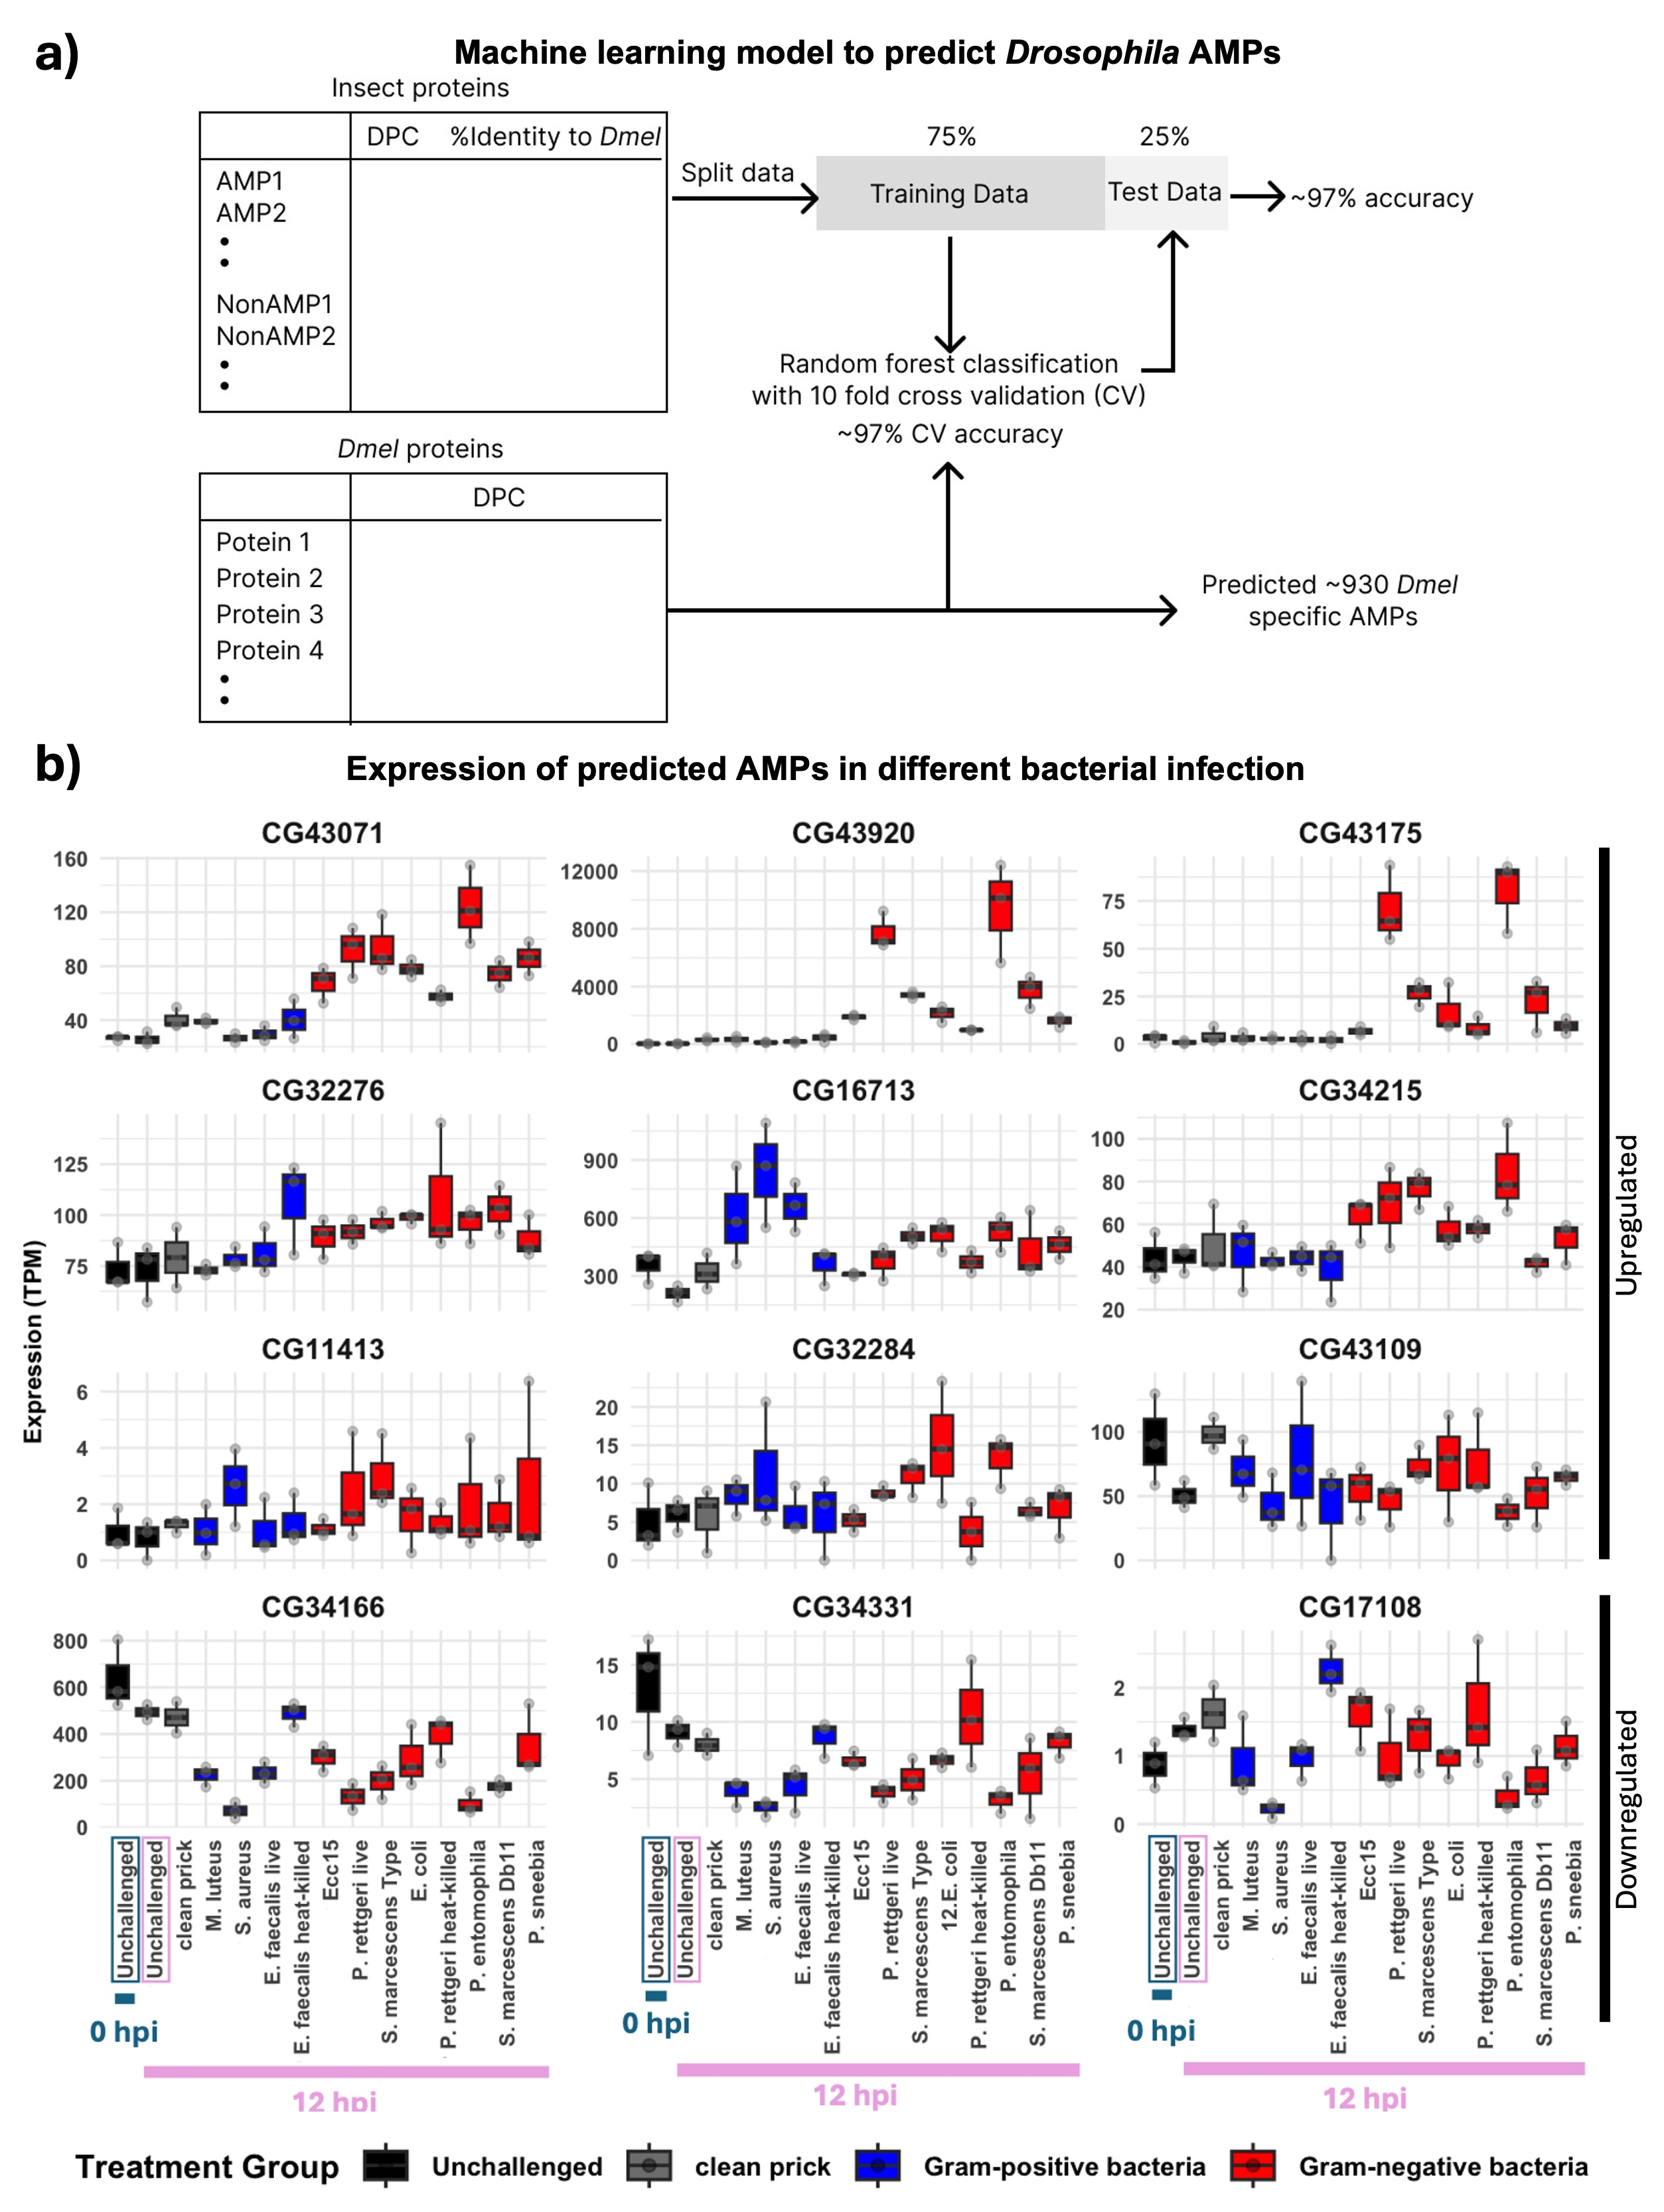
\includegraphics[width=1\textwidth]{figures/figure1.jpg}
    \caption{a. Workflow of the machine learning model (*DPC-Dipeptide protein composition), b. Expression of the predicted antimicrobial peptides (AMPs) in different bacterial infections.}
    \label{fig:figure1}
\end{figure}

\noindent to do functional studies these predicted AMPs by our model will help to narrow down the targets to choose from and to do functional studies on. Altogether, this study aims to identify new AMPs which will further our knowledge of different types of AMPs and will help us understand how they protect organisms from different pathogens and bacteria. Identifying different types of AMPs and understanding their function and specificity can facilitate identifying therapeutic targets that will help to prevent infections.

There are 427 insect AMPs that are well documented. We used protein sequenced of all of these insect AMPs as out positive data. For creating the negative dataset we carefully picked 459 non AMP insect protein sequences. In the Uniprot database these non AMP proteins did not have AMP, membrane, toxic, secretory, defensive, antibiotic, anticancer, antiviral, and antifungal keywords in their description. From the protein sequences, we calculated dipeptide composition (DPC) to use that as our variable features. We also calculated percentage identity of these protein sequences and used that as another variable in the final dataset to draw a relationship of these sequences to \textit{Drosophila} as our aim is to predict AMPs specific to \textit{Drosophila}. We chose insect known AMPs and non AMPs instead of only focusing on \textit{Drosophila} because we only know 25 AMPs in \textit{Drosophila}. Only 25 observations are not enough data to build a machine learning model. The final dataset had 886 observations (427 AMP and 459 non AMP). We splitted our dataset to use 75 percent of the data for machine learning model training and 25 percent as test data. We applied a variety of classification based machine learning model and we found that Random forest is working best with 3.163727 percent cross validation error rate. We found that it performed well in the testing data as well with 3.153153 percent error rate. The workflow diagram in shown in figure 1a. The similarity of error rate between cross validation and test data indicate the model is not overfitted. For further evaluating our model, we calculated accuracy, precision, AUC, recall, F1, and log loss matrices (Supplementary Materials). We found high accuracy and F1 score which indicate robust overall performance of the model. We also found high precision and recall showing that the model effectively manages false positives and false negatives. In our model, the AUC is close to 1 means the model performing excellent at distinguishing between AMP and non-AMP proteins. A low Log loss in the model suggests confident and accurate predictions of our random forest model for predicting AMPs. Then, we used all the \textit{Drosophila} proteins and calculated the dipeptide composition of the proteins and applied the data in our built random forest based machine learning model. The model predicted 930 \textit{Drosophila} specific AMPs (refer to supplementary data). As stated earlier \textit{Drosophila} has 25 well characterized AMPs. Among these 25 the model successfully predicted 23 of them (refer to supplementary data). To further screen the predicted 930 AMPs, we used an mRNA expression dataset where \textit{Drosophila} were exposed to different type of bacterial infection. By cross-referencing the AMPs predicted by our model with genes found to be differentially expressed in mRNA expression studies of bacterial infections, we identified 12 AMPs that met both criteria. The expression pattern of these 12 AMPs in bacterial infection is shown in figure 2b. The predicted AMPs CG43071, CG43920, CG43175, CG32276, CG16713, CG34215, CG11413, CG32284, CG43109 are mostly upregulated in bacterial infection but their specificity is different based on gram positive and negative bacteria. The predicted AMPs CG34166, CG34331, CG17108 are mostly downregulated. These 12 predicted AMPs have unknown function mostly. But now we know that they have possible antimicrobial functionality. Altogether, with the help of machine learning and mRNA expression based molecular study we screen predicted 12 possible genes that may have antimicrobial activity.

\section{Methods}
For calculating dipeptide composition of the insect proteins we used the tool ProFeatX. Percent identity of the insect sequences to \textit{Drosophila} was calculated using BLAST+. The protein sequences were download from UniProt database. The machine learning model, data analysis and visualization were done using R and R specific packages (tidyverse, reshape2, rpart, randomForest, ipred, caret, ROCR, pROC). The detailed code is give at github. 
%The analysis used a linear model to fit data from a simple dataset.
%Here is an example citation: \cite{Lamport1986}.

\bibliographystyle{apacite}
\bibliography{references}

\end{document}